% Point d'avancement tuteur, 24 juillet 2026. Compile avec Tectonic (pdfLaTeX standard).
% Perimetre : continuite directe du point du 17/07. Centre sur le rdv avec Mehdi Cherkaoui.
% Volontairement modeste : on ne saute pas d'etapes, les developpements avances (branchement,
% Hawkes, Poisson compose, cas d'usage detailles) sont gardes pour un point ulterieur.
\documentclass[11pt]{beamer}
\usetheme{Madrid}
\usecolortheme{seahorse}
\usepackage[utf8]{inputenc}
\usepackage[T1]{fontenc}
\usepackage[french]{babel}
\usepackage{booktabs}
\usepackage{eurosym}
\graphicspath{{../vasicek_lab/figures/}{../cascade_qualitative/figures/}}
\setbeamertemplate{navigation symbols}{}
\setbeamertemplate{caption}{\raggedright\insertcaption\par}
\setbeamerfont{block title}{size=\small}

\title[Point d'avancement]{Mémoire SCR DORA : point d'avancement}
\subtitle{Suites du 17/07 et échange avec Mehdi Cherkaoui}
\author[K. Kaddouri]{Kélian Kaddouri}
\institute[ENSAE / Nexialog]{ENSAE / Nexialog Consulting}
\date[24/07/2026]{24 juillet 2026}

\begin{document}

\begin{frame}
\titlepage
\end{frame}

% =====================================================================
\begin{frame}{Ce qu'on s'était dit la dernière fois}
Au point du 17/07, trois pistes pour la suite :
\begin{enumerate}
\item \textbf{Valider les jugements de base} du classeur (\texttt{ROOT}, \texttt{TRANS},
      \texttt{GBASE}) et le traitement du gain de contagion $g$.
\item \textbf{Brancher le modèle sur des sévérités}, pour passer de la lecture ordinale
      à une lecture quantitative.
\item Si accessible, \textbf{explorer la piste d'un registre d'incidents} pour une première
      calibration de $W$ (la contagion dirigée entre piliers).
\end{enumerate}
\medskip
Et, en fin de call, une piste \textbf{fréquence d'entrée} à creuser (avec Coraline).
\vfill
\begin{block}{}
Ce point avance surtout sur le \textbf{3\ieme} : la réponse est arrivée, par l'échange avec
Mehdi. Elle est \textbf{négative mais utile}. Plus un premier pas côté données.
\end{block}
\end{frame}

% =====================================================================
\begin{frame}{Le cœur du mémoire : le modèle de cascade}
Un sinistre ne reste pas dans un pilier : une défaillance \textbf{se propage de pilier en
pilier, en suivant un ordre}. Le mémoire modélise cette \textbf{chaîne dirigée}, à partir
de trois jugements d'expert.
\begin{itemize}
\item \texttt{ROOT} : propension d'un pilier à \textbf{amorcer} la cascade.
\item \texttt{TRANS} : force du maillon \og{}$i$ entraîne $j$\fg, \textbf{asymétrique}
      ($i\!\to\!j \neq j\!\to\!i$). C'est la brique qui porte la \textbf{direction}.
\item \texttt{GBASE} : gravité propre de chaque pilier, \textbf{composée} le long de
      l'ordre (des défaillances qui s'enchaînent s'aggravent).
\end{itemize}
La \textbf{criticité} croise probabilité et gravité, lue en catégories.
\vfill
\begin{block}{La signature : la dépendance à l'ordre}
Mêmes piliers, ordre inverse, \textbf{verdict inverse} : P1$\to$P2 ressort Majeure,
P2$\to$P1 ressort Faible. Sur 26 ensembles de piliers, \textbf{22 changent de criticité
selon l'ordre}. Une corrélation, symétrique, ne peut pas le reproduire.
\end{block}
\end{frame}

% =====================================================================
\begin{frame}{La même cascade, en quantitatif : le Vasicek dirigé}
La cascade qualitative est injectée dans le modèle de capital. Le stress latent du pilier
$j$ d'une entité combine trois briques :
\[
X_{ij} \;=\; \underbrace{\sum_{k\neq j} W_{jk}\,X_{ik}}_{\text{contagion dirigée}}
   \;+\; \underbrace{\sqrt{\rho_{ij}}\;Y_j}_{\text{systémique}}
   \;+\; \underbrace{\sqrt{1-\rho_{ij}}\;\varepsilon_{ij}}_{\text{propre}}
\]
\begin{itemize}
\item $W$ est bâtie depuis \texttt{TRANS} et normalisée à la Leontief
      ($W = g\,\texttt{TRANS}/\max_j \sum_k \texttt{TRANS}_{jk}$), d'où $\rho(W)\le g<1$ :
      la stabilité est garantie par construction.
\item Forme réduite : $\mathbf{X}_i = (I-W)^{-1}\,(\text{systémique} + \text{propre})$.
\end{itemize}
\vfill
\textbf{Rien n'a bougé sur l'ossature.} Ce point ne touche pas le modèle : il porte sur
\textbf{ce qu'on peut, ou non, calibrer dessus}.
\end{frame}

% =====================================================================
\begin{frame}{La cascade est un processus de branchement multitype}
\small
Le bon objet dynamique porte sur les \textbf{incidents} (contagion retardée), non sur les
latentes simultanées. Avec $\text{base}_j$ le seuil reporté côté stress et $s_j$ la charge
systémique du pilier :
\[
X_{ij,t} = \text{base}_j + \sum_{k\neq j} W_{jk}\,D_{ik,t-1} + s_j\,Y_{j,t}
           + \varepsilon_{ij,t},
\qquad D_{ij,t} = \mathbf 1\{X_{ij,t} \ge 0\}.
\]
Un incident sur $k$ engendre à la période suivante des incidents ailleurs. L'objet central
n'est plus $W$ mais la \textbf{matrice de génération suivante} $M$, qui compte des
incidents :
\[
M_{jk} = \underbrace{\Phi(\text{base}_j + W_{jk})}_{\text{incident en } j \text{ si } k \text{ a frappé}}
       - \underbrace{\Phi(\text{base}_j)}_{\text{proba de fond}},
\qquad R_0 = \rho(M).
\]
\begin{itemize}
\item La cascade \textbf{s'éteint si et seulement si $R_0 < 1$} (le $R_0$ des
      épidémiologistes), à ne pas confondre avec $\rho(W)<1$, qui gouverne le système
      \emph{latent simultané}.
\item $(I-M)^{-1}$, la \textbf{progéniture totale attendue}, reproduit \emph{exactement} le
      classement \texttt{ROOT} (Spearman $=1{,}00$) : \texttt{ROOT} en devient redondant.
\end{itemize}
\end{frame}

% =====================================================================
\begin{frame}{L'échange avec Mehdi Cherkaoui}
Avant son départ, un cadrage \textbf{métier} sur la lecture opérationnelle du sujet.
\begin{itemize}
\item DORA s'applique aux \textbf{institutions financières} : bien s'imprégner des
      subtilités du texte, et viser un \textbf{cas d'usage} concret plutôt que de rester
      au niveau général.
\item Le message central : \textbf{\og{}tu ne pourras pas tester la contagion entre les
      différents piliers, c'est trop compliqué\fg{}}.
\item Le \textbf{pilier 4 (tiers)} est souvent le \textbf{point d'entrée le plus critique}
      : registre d'externalisation, mapping des sous-traitants, un prestataire qui tombe
      et impacte toutes les activités de la banque. C'est \og{}le trou dans la raquette\fg.
\item Conseil données : plutôt que le général, cibler \textbf{P2 / P3 / P4} et chercher
      de la donnée \textbf{open source}.
\end{itemize}
\end{frame}

% =====================================================================
\begin{frame}{Pourquoi c'est une bonne nouvelle}
\og{}On ne pourra pas tester $W$\fg{} \textbf{est exactement ce que mon étude de
faisabilité avait déjà montré}, chiffres à l'appui : aucune source publique ne code les
piliers co-touchés avec un horodatage fin, et l'asymétrie directionnelle tombe sous le
test placebo.
\vfill
\begin{block}{}
Un praticien arrive \textbf{par l'intuition métier} à la conclusion que j'avais établie
par une analyse quantitative. Ce n'est pas une menace pour le mémoire : c'est une
\textbf{validation externe d'une limite que je documente déjà}, et l'objection d'un
praticien anticipée avant la soutenance.
\end{block}
\end{frame}

% =====================================================================
\begin{frame}{Ce que ça change, et ce que ça ne change pas}
\textbf{Ce qui ne change pas.} La cascade reste le \textbf{modèle normatif} : jugement
d'expert assumé, exploré en sensibilité. C'est la direction validée le 17.
\medskip

\textbf{Ce qui change.} Le \textbf{poids empirique} ne se met plus sur $W$ (inidentifiable),
mais \textbf{par pilier}, là où la donnée existe. La contagion inter-piliers reste
conceptuelle ; le chapitre empirique se construit à côté.
\vfill
\begin{block}{Le cas d'usage ne fait pas quitter le cadre}
Se resserrer sur un cas d'usage (la piste de Mehdi) ne remplace pas le cadre général :
ma machinerie de criticité (ordre, \texttt{ROOT} / \texttt{TRANS} / \texttt{GBASE})
s'applique \textbf{à l'identique entre sous-process d'un même pilier}, là où la donnée
existe. Même modèle, une maille plus fine.
\end{block}
\end{frame}

% =====================================================================
\begin{frame}{Comment on pallie le manque de donnée sur $W$}
\small
On ne calibre pas $W$, mais on ne le pose pas en aveugle non plus. \textbf{Trois leviers.}
\begin{enumerate}
\item \textbf{Séparer l'identifiable du reste.} $W = S + A$ : la partie symétrique $S$
      (co-occurrence de piliers, que la donnée \emph{voit}) est \textbf{identifiée} ;
      seule la partie antisymétrique $A$, la \textbf{direction}, ne l'est pas. Le manque
      ne porte que sur $A$, pas sur tout $W$.
\item \textbf{Borner plutôt que poser, et lire le SCR en fourchette.} On encadre
      l'ignorance directionnelle ($|A_{jk}| \le t\,S_{jk}$) et on balaie tout l'ensemble
      admissible. Le socle sans contagion et la co-occurrence fixent déjà
      \textbf{l'essentiel} du capital ; la direction ne joue que sur une \textbf{bande}.
      \textbf{Le SCR devient une fonction de $W$, pas un point.}
\item \textbf{Resserrer par élicitation structurée (méthode de Cooke).} Un panel
      d'experts fournit la direction, \textbf{pondéré par des questions-graines} dont je
      connais déjà la réponse (mes chapitres empiriques) : des avis \emph{calibrés}, pas
      crus sur parole. L'élicitation ne sert qu'à départager les piliers de tête.
\end{enumerate}
\textbf{Ligne rouge} : ne jamais présenter $W$ comme calibré. La non-identifiabilité, et
la spécification du registre horodaté qu'il faudrait, sont elles-mêmes un \textbf{livrable}.
\end{frame}

% =====================================================================
\begin{frame}{Un premier pas côté données : la fréquence d'entrée}
\begin{center}
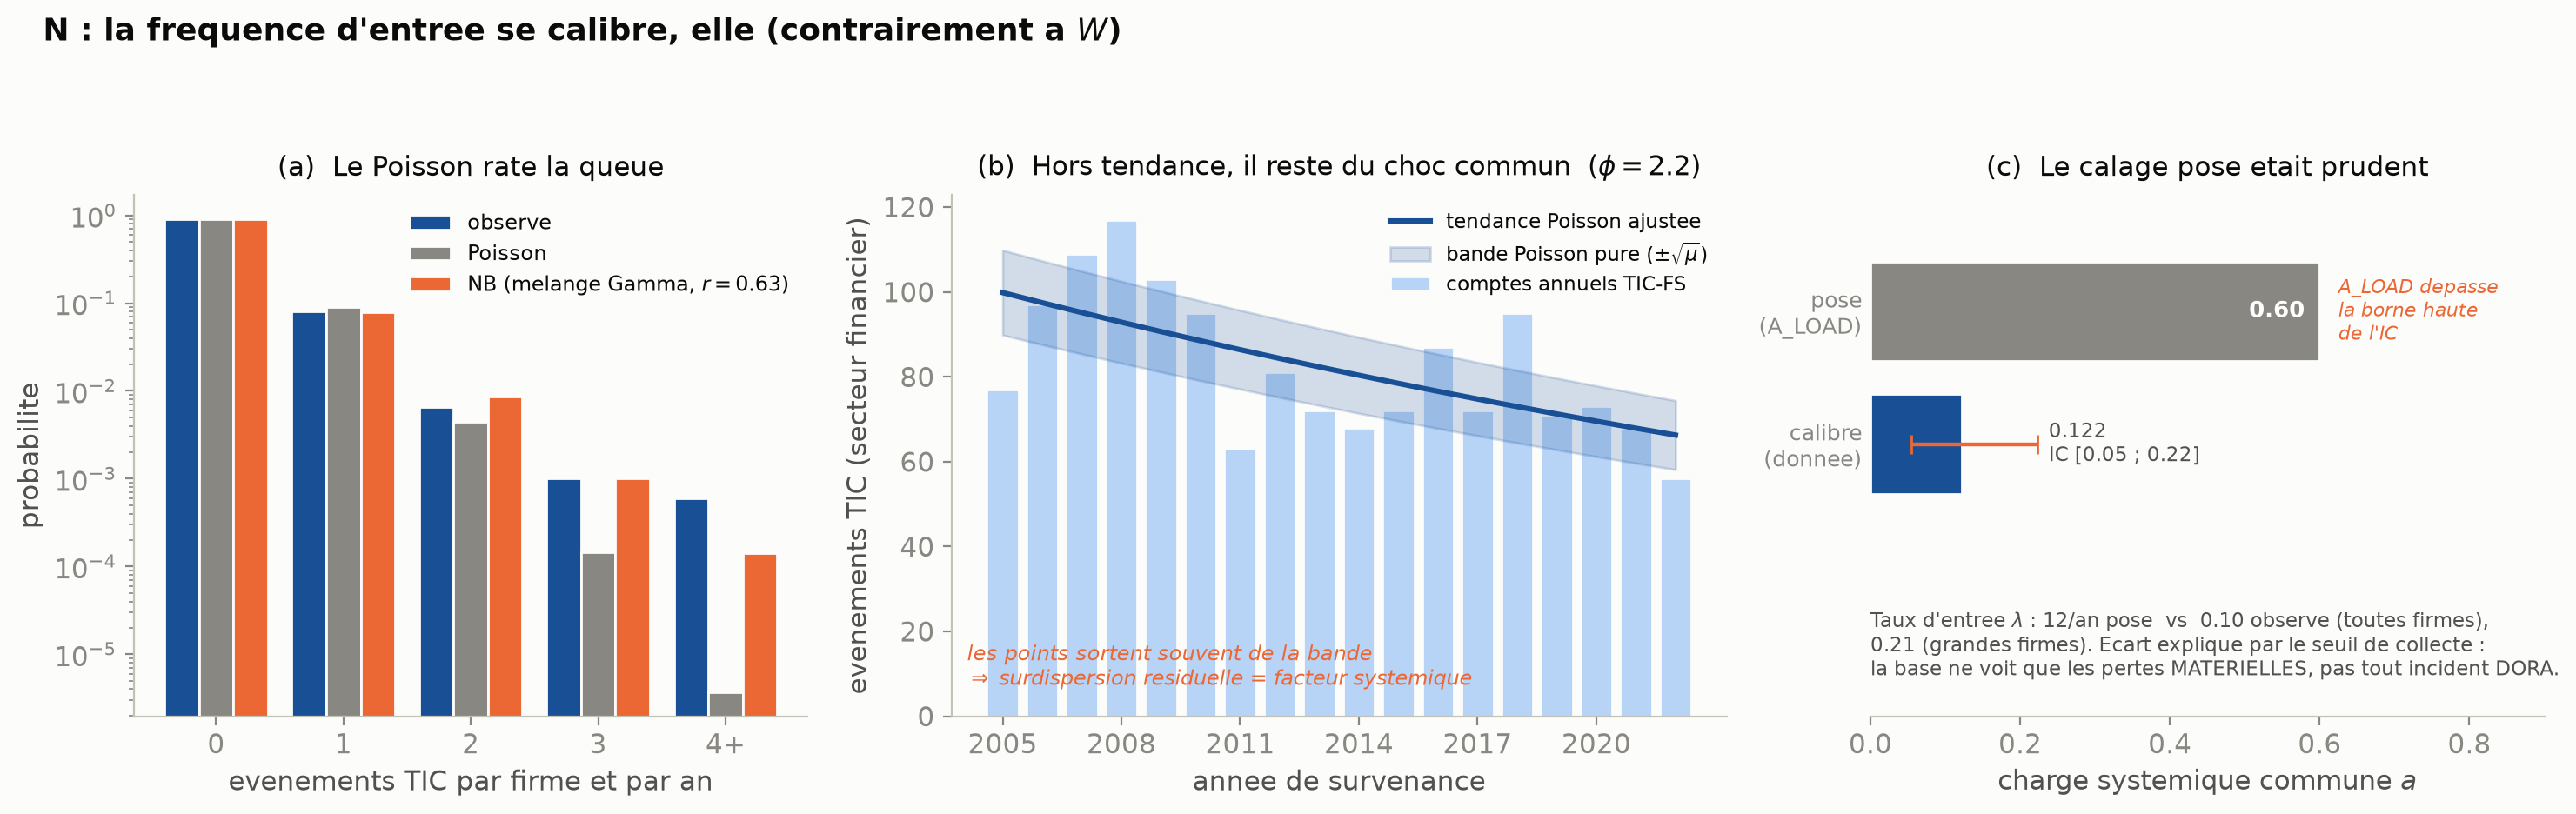
\includegraphics[width=0.92\linewidth]{N_frequence_entree.png}
\end{center}
Sur le SAS OpRisk (TIC, secteur financier), première calibration de l'\textbf{étage
fréquence} : le Poisson simple est rejeté, la loi est \textbf{surdispersée}. La charge
systémique observée est \textbf{nettement en dessous} de la valeur que j'avais posée : le
calage actuel est \textbf{conservateur}, et je peux désormais le \textbf{chiffrer} plutôt
que de le supposer. C'est le sens du 17 : \og{}brancher le modèle sur des données\fg.
\end{frame}

% =====================================================================
\begin{frame}{La piste de Mehdi : un cas d'usage par pilier}
Le score de criticité, abstrait, doit se \textbf{traduire en KPI observables} sur donnée
ouverte. Une \textbf{première lecture} (à approfondir) par pilier :
\begin{center}\footnotesize
\renewcommand{\arraystretch}{1.35}
\begin{tabular}{@{}l l l@{}}
\toprule
\textbf{Pilier} & \textbf{KPI candidat} & \textbf{Ordre de grandeur} \\
\midrule
P2 incidents  & délai de notification & médiane $\sim$3 mois ; majorité $>$ 1 mois (art.~19) \\
P3 résilience & temps de containment  & médiane $\sim$1 semaine ; queue $>$ 90 j \\
P4 tiers      & concentration         & une poignée de jours porte 20\,\% des pertes \\
\bottomrule
\end{tabular}
\end{center}
\vfill
\textbf{Convergence indépendante} : la donnée place l'accumulation sur les \textbf{tiers}
(P4), là où le classeur, par pur jugement d'expert, mettait \textbf{déjà} P4 en tête
($\texttt{ROOT}[4]=0{,}90$). Deux chemins distincts, un même pilier. Et ce chapitre
\textbf{ne dépend pas de $W$}.
\end{frame}

% =====================================================================
\begin{frame}{Points bloquants et pour la prochaine fois}
\small
\textbf{Ce qui reste ouvert}
\begin{itemize}
\item La bande sur $W$ ne se resserre que par \textbf{l'élicitation}, à mener avec les
      experts ; le \textbf{registre horodaté} taxonomisé par pilier reste la donnée qui
      manque pour trancher la direction.
\item Le \textbf{choix du KPI} et de la définition de l'\og{}incident significatif\fg{}
      (impact financier ou réputationnel) à figer par pilier.
\end{itemize}
\textbf{Pour la prochaine fois}
\begin{itemize}
\item Approfondir un \textbf{cas d'usage} (P4 semble le plus porteur) au niveau
      \textbf{sous-process}, sur les données que Mehdi doit fournir (registre
      d'externalisation).
\item Consolider le premier tableau de KPI par pilier et son lien au score de criticité.
\end{itemize}
\vfill
\begin{block}{}
Ligne de conduite : \textbf{continuité du 17}, pas de saut. La cascade est stable, le
travail se déplace vers \textbf{la donnée qui existe}, pilier par pilier.
\end{block}
\end{frame}

\end{document}
